% !TeX root =./main.tex
% !TeX spellcheck = en_US


Over-weight load, i.e., vehicles loaded with more than 11 tons per axle,
are even harder to plan then over-size load. Over-sized load is limited
by road turning radius, transportation corridor width and road-side obstacles, such as traffic lights, power lines. Hence planning is dominated these local characteristics
and in-person inspection of the suggest route.

In contrast to that, the planning process for over-weight includes the consultation
of an civil engineer who must determine the allowable weight and speed to pass
complex building structures such as bridges.
This time consuming process must be repeated once the intended route is determined infeasible or changes for any other reason.
In an attempt to relieve some of this cumbersome workload from civil engineers,
we propose an mathematical optimization approach.
This labour intense planning procedure is described in
\citet{Osegueda.1999}.

To this end, a mathematical model determines the optimal path between two
points within the road network while respecting the bridge capacity constraints.
This serves as an \textit{decision support system} for civil engineers.
Ultimately,  each route must be must be approved by a civil engineer  in terms of
bridge capacities and other structural limitations.

Under the assumption that the model generates feasible routes,
we conduct a study that compares several (possibly conflicting) objectives.
Therefore, we consider different types of vehicles and different loads.

Possible objective are:
\begin{itemize}
  \item Shortest Path (classic).

  \item Minimal wear of infrastructure. Reducing the wear induced by over-weight transports
  minimizes maintenance costs, extends lifetime of the building structures, and
  improves safety (Genoa bridge collapse in 2018).

  \item Minimize the number of different road operators and municipalities the path
  traverses. In that sense, the process of getting official approval of the
  path should be simplified.
\end{itemize}

\section{Related Work}



\subsection{Morandi Bridge Colapse}

\cite{Morgese.2020}
\cite{MorandiNYTimes}


\section{Commercial Solutions}

\subsection{HERE}
\url{https://www.here.com/}

\subsection{Bentley Superload Routing}
\url{https://www.bentley.com/en/products/product-line/asset-performance/superload-routing}



\section{Matrix Representation of the Road Network}

For now, we consider the \textit{higher level road network} in Carinthia,
i.e., \textit{A}, \textit{S}, \textit{L}, \textit{B}, in form of a matrix.
The vertices of the matrix are the crossing points of the roads, while
the road section connecting those points form the edges of the matrix.
For each edge, we have the distance between the vertices and the length of the bridges along the segment and the capacity constraints (and the lowest encountered bridge capacity) for each edge.
This way, we can answer various questions concerning transports between those vertices.



\begin{figure}
 \centering
  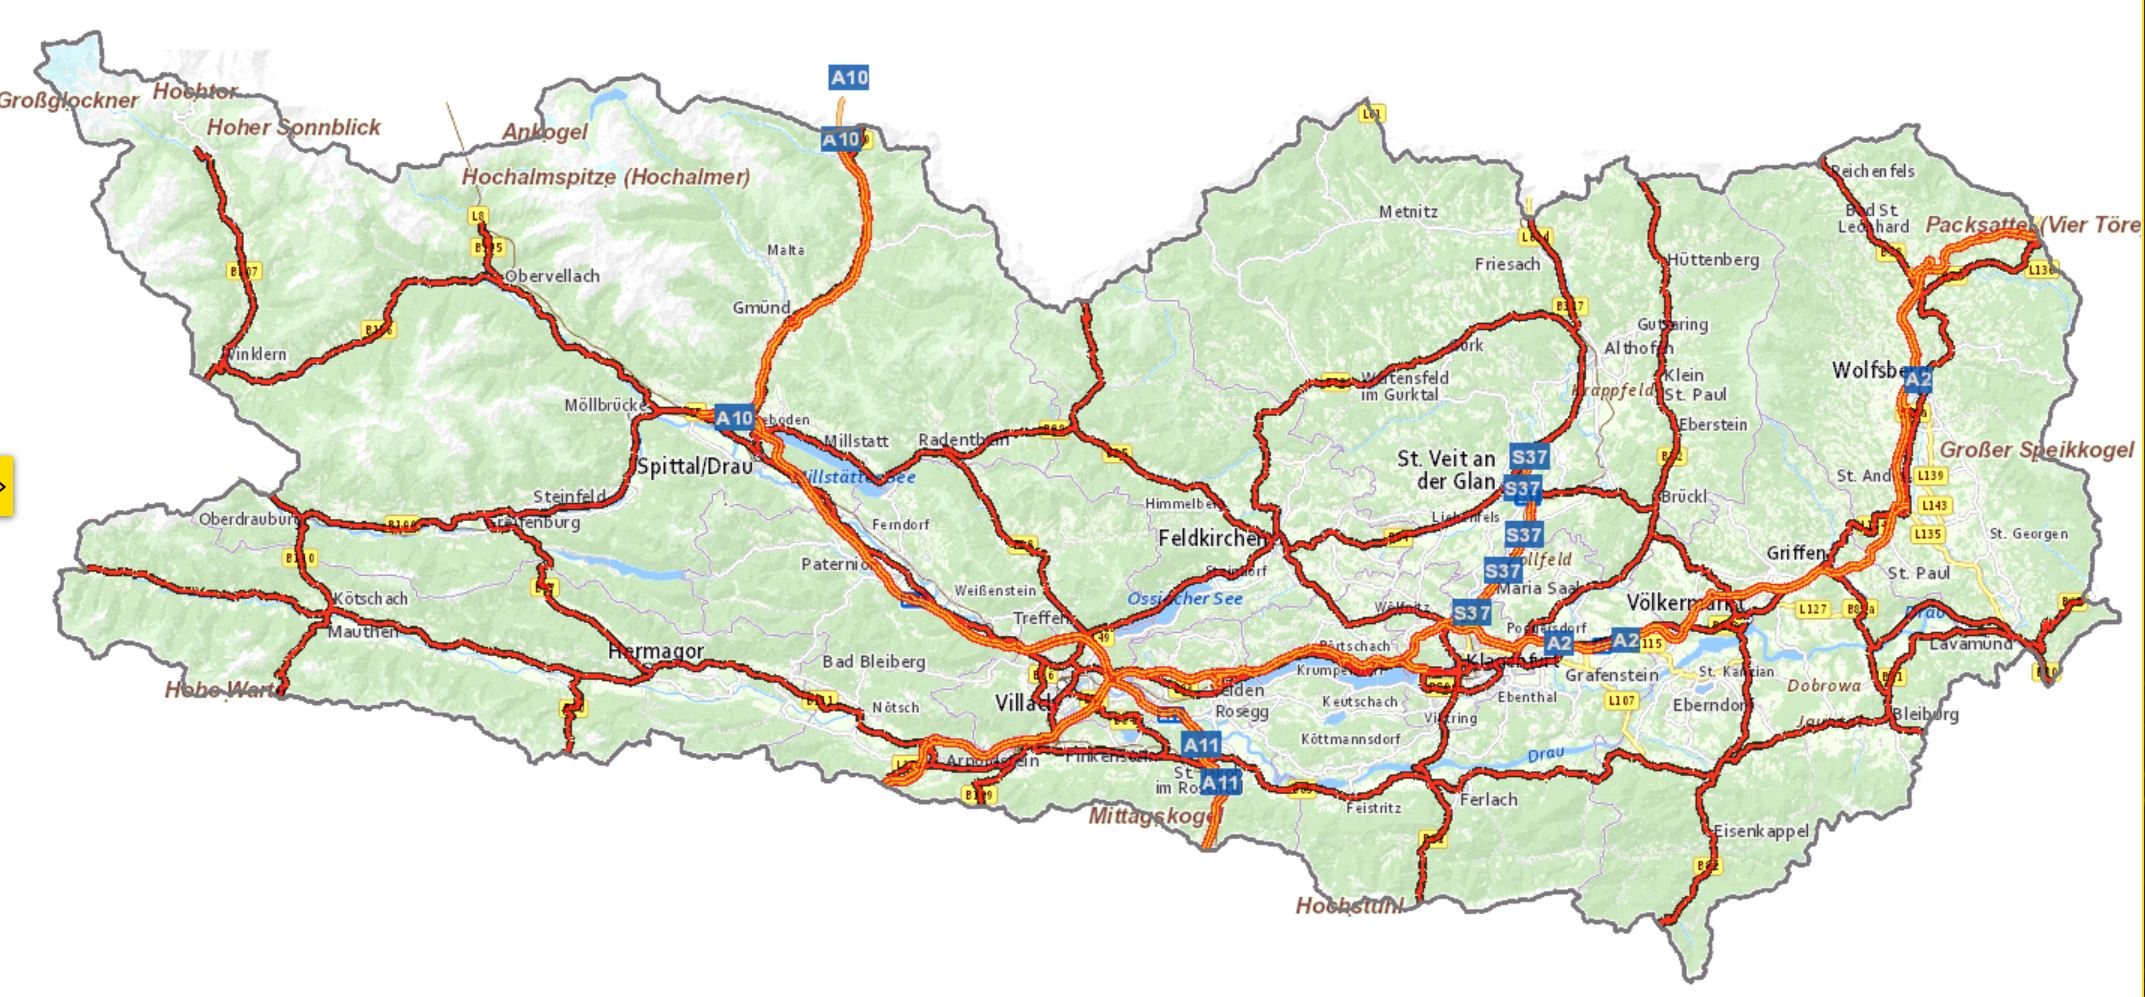
\includegraphics[width=0.9\textwidth]{map.jpg}
  \caption{Overview of the higher level road network in Carinthia.}
  \label{fig:higher level}
\end{figure}
